\documentclass[a5paper]{article}
\usepackage[a5paper, top=8mm, bottom=8mm, left=8mm, right=8mm]{geometry}

\usepackage{polyglossia}
\setdefaultlanguage[babelshorthands=true]{russian}

\usepackage{fontspec}
\setmainfont{FreeSerif}
\newfontfamily{\russianfonttt}[Scale=0.7]{DejaVuSansMono}

\usepackage[font=scriptsize]{caption}

\usepackage{amsmath}
\usepackage{amssymb,amsfonts,textcomp}
\usepackage{color}
\usepackage{array}
\usepackage{hhline}
\usepackage{cite}

\usepackage[hang,multiple]{footmisc}
\renewcommand{\footnotelayout}{\raggedright}

\PassOptionsToPackage{hyphens}{url}\usepackage[xetex,linktocpage=true,plainpages=false,pdfpagelabels=false]{hyperref}
\hypersetup{colorlinks=true, linkcolor=blue, citecolor=blue, filecolor=blue, urlcolor=blue, pdftitle=1, pdfauthor=, pdfsubject=, pdfkeywords=}

\usepackage{tabu}

\usepackage{graphicx}
\usepackage{indentfirst}
\usepackage{multirow}
\usepackage{subfig}
\usepackage{footnote}
\usepackage{minted}

\sloppy
\pagestyle{plain}

\title{Базы данных}
\author{Юрий Литвинов\\\small{yurii.litvinov@gmail.com}}

\date{12.10.2018г}

\begin{document}

\maketitle
\thispagestyle{empty}

\section{Введение}

Без работы с базами данных не обходится ни одно веб-приложение и вообще ни одно приложение, которому надо что-то долго хранить и быстро получать доступ к данным. В принципе, люди долгое время прекрасно обходились обычными файлами, да и для задач типа хранения настроек приложения обычные файлы конфигурации вполне подходят. Но данные часто имеют сложную структуру, к ним приходится выполнять кучу разных видов запросов, к тому же данных, если они заводятся в вашем приложении, быстро становится очень много и они перестают помещаться в оперативке.

Кстати, есть базы данных, а есть системы управления базами данных, нехорошо их путать. БД --- это, собственно, данные вместе с их структурой, СУБД --- это программа, которая предоставляет к этим данным доступ и позволяет их редактировать (или их структуру). СУБД бывают концептуально разные, каждый подход имеет свои достоинства и недостатки:

\begin{itemize}
	\item Реляционные --- до сих пор самый популярный вид СУБД, использующий реляционную алгебру (\url{https://en.wikipedia.org/wiki/Relational_algebra}) для представления данных и операций над ними. Данные в реляционной модели представляются в виде \textit{кортежей} значений разных типов, объединённых в \textit{отношения} --- самые настоящие алгебраические отношения и кортежи, в простонародье называемые таблицами и строками. На отношениях определены алгебраические операции, которые принимают отношения и возвращают отношения, определены совершенно формально и их свойства хорошо изучены. Эти алгебраические операции выражаются операторами языка SQL, который достаточно прост, чтобы им мог пользоваться любой школьник, несмотря на то, что внутри происходит кошмарная алгебраическая наука. Операции достаточно выразительны, чтобы с данными можно было делать практически всё, что угодно, и при этом достаточно декларативны, чтобы СУБД могла сама решать, как исполнять запрос, оптимизируя его зачастую в тысячи раз по сравнению с наивной реализацией.
	\item Объектно-ориентированные --- хранят по сути сериализованные объекты и позволяют исполнять запросы в духе ``найти объект по шаблону''. Значительно менее выразительный язык запросов компенсируется удобством использования из объектно-ориентированных программ --- результатом операции становится не какой-то невнятный набор кортежей, которые ещё надо как-то загрузить в объектно-ориентированную модель, а самый настоящий объект, будто мы его хранили в памяти. К тому же, такие базы, как правило, проще в конфигурировании и использовании, так что очень популярны сейчас для хранения небольших объёмов данных или данных, не предполагающих сложных запросов.
	\item Иерархические --- СУБД, хранящие данные в виде дерева. Самый типичный нынче пример таких штук --- базы, хранящие данные в XML-документах. Для запросов там используется язык XQuery, работающий с выражениями на языке XPath. Для иерархических по своей природе данных такие штуки незаменимы.
	\item Другие --- например, дедуктивные базы данных, которые вообще не хранят данные, они хранят некоторый набор фактов и правила, по которым могут быть выведены остальные факты (например, см. \url{https://en.wikipedia.org/wiki/Datalog}). 
\end{itemize}

Наиболее популярны сейчас всё-таки реляционные и объектно-ориентированные базы данных, поэтому часто приходится решать, какую же из этих моделей использовать. Так что рассмотрим соображения, могущие повлиять на решение:
\begin{itemize}
	\item Реляционные
	\begin{itemize}
		\item Минусы --- сложность интеграции с объектно-ориентированным кодом. Реляционная модель данных концептуально построена по принципу ``сущность-связь'', где сущность --- это штука, у которой есть имя и атрибуты, могущие иметь значения, а связь --- это ссылка из одной сущности на другую. Это очень похоже на объекты и отношения между ними, так что, казалось бы, никаких пробелм быть не должно, но нет: сущности не могут наследоваться, друг от друга, например. Чтобы хранить в реляционной базе объекты двух разных классов, наследующихся от общего предка, потребуется либо две таблицы с атрибутами, куда раскопипащены атрибуты предка, либо три таблицы --- для предка и двух потомков, и явные связи между потомками и предком. При загрузке и сохранении таких ``объектов'' фактически приходится реализовывать наследование вручную. Ещё реляционные базы не могут в отношение ``многие ко многим'', потому что связь там --- это просто ссылка на строку в другой таблице, она может быть только одной. Для решения этой проблемы заводят вспомогательные ``таблицы-развязки'', хранящие в себе только набор связей.
		\item Плюсы --- выразительный язык запросов, который даже со всякими там таблицами-развязками позволяет выбрать именно те данные, что нужны, и представить их в более-менее удобном виде. Кроме того, запросы выполняются, как правило, очень эффективно, грамотный проектировщик схемы БД может сделать так, чтобы выборка из сотен гигабайт данных занимала всего доли секунды. Впрочем, неудачная схема БД может испортить скорость работы всего приложения очень серьёзно.
	\end{itemize}
\end{itemize}

\section{Реляционная модель данных}

Рассмотрим подробнее реляционную модель (без алгебраических деталей). Данные там хранятся в виде отношений, которые удобнее всего себе представлять как таблицы, как на рисунке~\ref{image:table} из Википедии.

\begin{figure}
	\begin{center}
		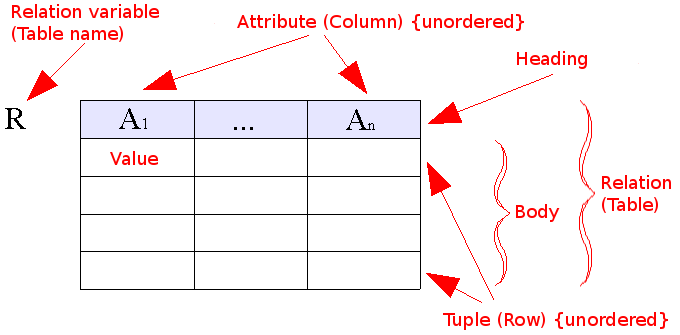
\includegraphics[width=0.7\textwidth]{relationalModel.png}
	\end{center}
	\caption{Отношение.}
	\label{image:table}
\end{figure}

У отношения есть имя (имя таблицы), у него есть колонки с именами и типами, и строчки, состоящие из, собственно, данных, лежащих в таблице. Пример таблицы с данными представлен в~\ref{table:tableWithData}.

\begin{figure}
	\begin{center}
		\begin{tabu} {| X[0.9 l p] | X[1 l p] | X[1 l p] | X[1 l p] |}
			\tabucline-
			CustomerID       & TaxID        & Name       & Address           \\
			\tabucline-
			\everyrow{\tabucline-}
			1234567890       & 555-5512222  & Munmun     & 323 Broadway      \\
			2223344556       & 555-5523232  & Wile E.    & 1200 Main Street  \\
			3334445563       & 555-5533323  & Ekta       & 871 1st Street    \\
			423242432        & 555-5325523  & E.F. Codd  & 123 It Way        \\
		\end{tabu}
	\end{center}
	\caption{Таблица с данными.}
	\label{table:tableWithData}
\end{figure}

\subsection{Ключи}

Если бы все данные, которые нужны программе, можно было хранить в одной таблице, то никакая реляционная алгебра и не нужна. Интереснее становится, когда данные имеют сложную структуру, требующую нескольких связанных таблиц. Например, список городов и список улиц, где каждая улица привязана к конкретному городу (рис.~\ref{table:citiesStreets})

\begin{figure}
	\begin{center}
		CITY
		\begin{tabu} {| X[0.2 l p] | X[1 l p] |}
			\tabucline-
			ID      & Name \\
			\tabucline-
			\everyrow{\tabucline-}
			1       & Москва \\
			2       & Санкт-Петербург \\
			3       & Владивосток \\
		\end{tabu}
		\vspace{3mm}
		STREET
		\begin{tabu} {| X[0.2 l p] | X[1 l p] | X[0.7 l p] |}
			\tabucline-
			ID       & Name             & ID\_CITY \\
			\tabucline-
			\everyrow{\tabucline-}
			181      & Малая Бронная    & 1 \\
			182      & Тверской Бульвар & 1 \\
			183      & Невский проспект & 2 \\
			184      & Пушкинская       & 2 \\
			185      & Светланская      & 3 \\
			186      & Пушкинская       & 3 \\
		\end{tabu}
	\end{center}
	\caption{Таблицы с городами и улицами.}
	\label{table:citiesStreets}
\end{figure}

В принципе, всё можно было сложить и в одну таблицу (хранить в STREET просто названия городов), но, во-первых, это дупликация данных, во-вторых, города могут понадобиться кому-то ещё.

Как в базах данных работают ссылки на другие таблицы --- очень просто, на самом деле. Есть понятие ``ключ'', набор столбцов, уникально идентифицирующих любой кортеж в таблице. Превичный ключ --- это уникальный идентификатор в таблице с нашими данными, внешний ключ --- это уникальный идентификатор наших данных, сохранённый в какой-то другой таблице. В примере~\ref{table:citiesStreets} первичным ключом в таблице CITY был столбец ID, в таблице STREET тоже есть первичный ключ (и тоже ID), но есть и внешний ключ --- столбец ID_CITY, где просто записаны первичные ключи городов, которым принадлежат улицы. 

Может показаться, что первичный ключ --- это всегда число, что-то вроде номера ячейки памяти, но нет, они бывают разные. Бывают естественные первичные ключи --- идентификаторы, присущие самим данным, например, номер паспорта или номер зачётки. Они уникальны по самой своей природе, поэтому вполне подходят в качестве первичных ключей. Бывают даже составные ключи --- ключи, состоящие из нескольких колонок. Например, название не идентифицирует город однозначно, но название страны, название региона плюс название города --- вполне себе уникальный идентификатор. Тогда в качестве внешнего ключа приходится использовать все значения, входящие в составной ключ.

Суррогатными ключами называются ключи, которых нет в предметной области, и их пришлось специально придумать, чтобы однозначно идентифицировать объекты (например, ID из~\ref{table:citiesStreets}). Они используюся чаще, чем естественные, потому что они заведомо уникальны --- например, MAC-адрес было бы разумно использовать как естественный ключ, но только до тех пор, пока нам не попадутся две сетевые карты с одинаковым MAC-адресом, который должен быть глобально уникальным. Кроме того, они компактнее, чем большинство естественных ключей. Но не очень хорошо работают в сценариях, когда требуется использовать данные из двух разных баз данных, так что естественные ключи всё-таки бывают полезны.

\subsection{Ограничения}

Базе данных можно сказать, что колонка --- это первичный ключ, тогда она будет сама проверять его уникальность (и даже генерить, если попросить). Это делается с помощью \textit{ограничений} --- свойств колонок в схеме БД. Первичные ключи описываются как ограничение PRIMARY KEY (чуть попозже будет понятно, куда это писать). Бывает ещё ограничение FOREIGN KEY, заставляющее СУБД проверять, что такой ключ действительно есть в таблице, на которую ссылается внешний ключ (сам ключ не ссылается, это просто значение, но в самом ограничении можно указать, о какой таблице идёт речь). Отметим, что кортеж, на который ссылается какой-то из внешних ключей, нельзя удалить (без \textit{каскадного удаления}, по крайней мере, когда удаляется и кортеж, и все кортежи, которые на него ссылаются, и все кортежи, которые ссылаются на них, и т.д.).

Есть ещё ограничение NOT NULL, заставляющее атрибут всегда иметь значение (по умолчанию значение любого типа может быть NULL, что означает отсутствие значения), и UNIQUE, что заставляет значение быть уникальным в своей колонке. Попытка вставить данные, которые нарушают уникальность, будет отклонена СУБД.

\section{SQL}

Теперь, собственно, про то, как работать с реляционными данными. Для этого чаще всего используется язык SQL (Structured Query Language). Он был специально спроектирован так, чтобы быть максимально простым и похожим на разговорный английский. 

Самый известный, пожалуй, оператор SQL --- это SELECT (да, в SQL ключевые слова по традиции пишут капсом, хотя сам язык регистронезависимый, как Паскаль). SELECT позволяет выббрать данные по некоторому критерию из некоторой таблицы или некоторого набора таблиц, получив новую таблицу (это алгебраический оператор, мы хотим замкнутость, так что да, результат SELECT --- таблица). Несколько примеров из Википедии приведены на рис.~\ref{image:select}, подробное описание можно посмотреть на \url{https://www.w3schools.com/sql/sql_select.asp} (учтите, что почти каждая СУБД имеет свой диалект SQL, так что синтаксис и возможности могут немного различаться, но для часто используемых случаев всё будет работать везде).

\begin{figure}
	\begin{center}
		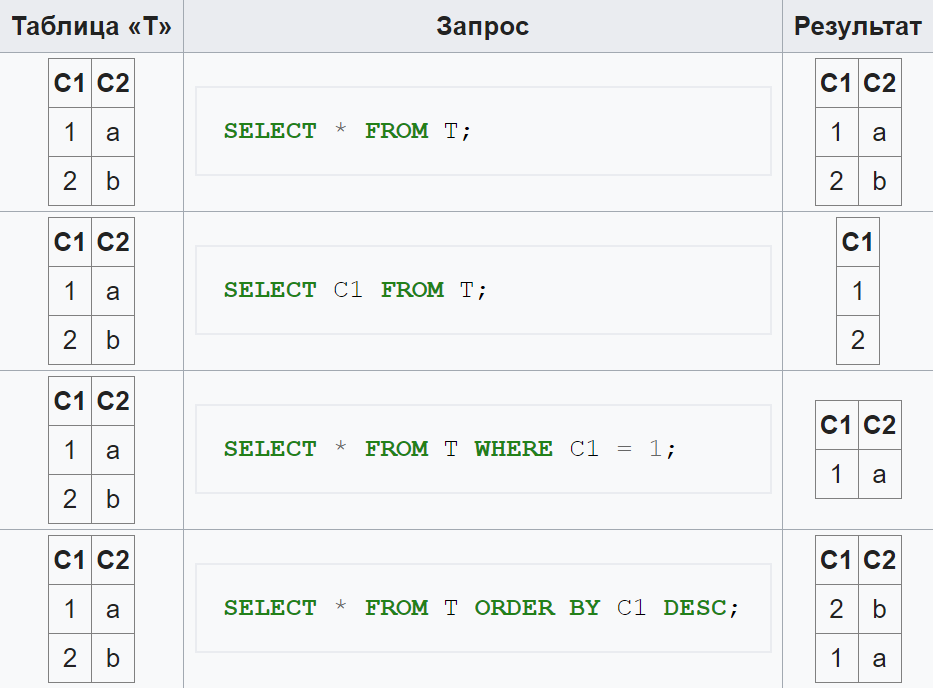
\includegraphics[width=0.5\textwidth]{select.png}
	\end{center}
	\caption{Оператор SELECT.}
	\label{image:select}
\end{figure}

Самое интересное тут, пожалуй, WHERE --- часть с предикатом, который определяет, какие кортежи попадут в результирующее отношение. Именно благодаря WHERE можно выбирать только те данные, которые нужны, и не грузить в оперативку все сотни гигов данных из базы.

Тестовая БД (MariaDB)
Устанавливаем MariaDB (https://downloads.mariadb.org/) 
При установке спросят пароль для пользователя root, придумываем, вводим и запоминаем его
Запускаем HeidiSQL, которая поставляется с MariaDB из коробки
“Создать” -> “Сеанс в корневой папке”
Вводим пароль для рута, который мы запомнили на этапе 1.а.
Порт 3306, по умолчанию.
Видим список баз, давайте создадим новую
Создаём тестовую БД, которую будем мучить
Правой кнопкой на Instance сервера (Unnamed), “Создать” -> “База данных”
Вводим имя БД, например, “myDB”, жмём “ОК”
База появилась в списке, создадим таблицу
Клик правой кнопкой по базе, “Создать” -> “Таблица”
Вводим имя (например, Cities)
Жмём “Добавить” рядом со “Столбцы”, вводим имя столбца (id) и тип данных (INT)
Снимаем галку “Разрешить NULL”
Ставим “По умолчанию” AUTO\_INCREMENT
Кликаем по нему правой кнопкой, “Создать новый индекс” -> “PRIMARY”
Добавляем второй столбец, name (типа VARCHAR(50))
Жмём “Сохранить”
Создадим вторую таблицу, People, со столбцами id, name и city\_id
Не забываем пометить id как AUTO\_INCREMENT и PRIMARY
Идём во вкладку “Внешние ключи”, жмём “Добавить”, пишем имя ключа “city\_id”, “Столбцы” – “city\_id”, “Справочная таблица” – “cities”, “Внешние столбцы“ – “id”
Добавим немного данных
“cities” -> “Данные”, правый клик, “Вставить строку”, игнорируем id, вводим “St. Petersburg” в name, кликаем куда-нибудь вне строки, строка добавилась
Вставляем ещё Moscow и ещё что-нить
“people” -> “Данные”, вставляем так же пару человек
Не забываем выбрать city\_id из списка, иначе операция добавления не пройдёт и вам напомнят
Пробуем написать SQL-запрос
Кликаем mydb, вкладку “Запрос”
Пишем там “SELECT people.name FROM people, cities WHERE people.city\_id = cities.id AND cities.name = "St. Petersburg"”
Жмём “Выполнить SQL” на панели инструментов
Видим таблицу с результатами нашего INNER JOIN-запроса снизу.

\end{document}
